%%% File encoding: UTF-8
%%% äöüÄÖÜß  <-- keine deutschen Umlaute hier? UTF-faehigen Editor verwenden!

\documentclass[master,german]{hgbthesis}
% Zulässige Class Options: 
%   Typ der Arbeit: diplom, master (default), bachelor, praktikum 
%   Hauptsprache: german (default), english
%%%----------------------------------------------------------

\RequirePackage[utf8]{inputenc}		% Bei der Verw. von lualatex oder xelatex entfernen!

\graphicspath{{images/}}    % Abbildungsverzeichnis
\logofile{logo}				% Name des Logo-PDFs in images/ (\logofile{}, wenn kein Logo gewünscht)
\bibliography{literatur}  	% Name der Biblatex-Literaturdatei (.bib)

%%%----------------------------------------------------------
% Angaben für die Titelei (Titelseite, Erklärung etc.)
%%%----------------------------------------------------------

%%% Einträge für ALLE Arbeiten: -----------------------------
\title{Serverlose und verteilte Softwarearchitektur in einer Microservice-Umgebung (V2)}
\author{Philipp Haider}
\studiengang{Software Engineering}
\studienort{Hagenberg}
\abgabedatum{2017}{07}{07}	% {YYYY}{MM}{DD}

%%% Zusätzlich für eine Bachelorarbeit: ---------------------
\nummer{1510454013}   % Stud-ID, z.B. 1310238045-A  
% (A = 1. Bachelorarbeit)
\semester{Sommersemester 2017} 
%\gegenstand{Einführung in die Tiefere Problematik 1} 
\betreuer{Johann Heinzelreiter, FH-Prof. DI} % oder \betreuerin{..}

%%% Restriktive Lizenformel anstatt CC (nur für Typ master) -
%\strictlicense

%%%----------------------------------------------------------
\begin{document}
%%%----------------------------------------------------------

%%%----------------------------------------------------------
\frontmatter                    % Titelei (röm. Seitenzahlen)
%%%----------------------------------------------------------

\maketitle
\tableofcontents

%\chapter{Kurzfassung}

Für die Realisierung von komplexen und skalierbaren Softwaresystemen ist ein Trend zur sogenannten Microservice"=Architektur, anstelle von monolithischen Architekturen zu beobachten. Bei diesem Architekturmuster handelt es sich um eine spezielle serviceorientierte Architektur, die aus tatsächlichen Anwendungsfällen von großen Internetfirmen hervorgegangen ist. In dieser Arbeit werden die Gründe für diesen Paradigmenwechsel gesucht und erläutert. Außerdem werden verschiedene Technologien für die erfolgreiche Umsetzung einer Microservice"=Architektur untersucht und miteinander in Verbindung gesetzt. Zu diesen Technologien zählen die Virtualisierung mit Containern, serverlose ereignisgesteuerte Funktionen und das Aktorenmodell. Auf Basis der genannten Konzepte gibt diese Arbeit Empfehlungen, für welche Szenarien der Microservices"=Ansatz überhaupt geeignet ist und wie dieser dann schlussendlich effektiv umgesetzt werden kann.		
%\chapter{Abstract}

\begin{english} %switch to English language rules

The development of complex and scalable software systems has shifted from monolithic architectures towards the so called microservice architecture. This architectural pattern has evolved out of real world use cases of large internet corporations as a variant of the service-oriented architecture. First, this thesis provides a survey of the reasons behind this paradigm shift. Furthermore different technologies for successfully implementing microservices are shown and compared to each other. Among those technologies are containers for virtualization, serverless event-driven functions and the actor model. Based on the enumerated concepts this thesis provides recommendations to find suited applications for microservices and describes how to effectively apply this architectural style to complex software systems.

\end{english}
			

%%%----------------------------------------------------------
\mainmatter          % Hauptteil (ab hier arab. Seitenzahlen)
%%%----------------------------------------------------------

\chapter{Microservices}

Der Begriff Microservices stiftet derzeit noch große Verwirrung. Nicht nur weil er relativ neu ist, sondern auch weil er sehr breit gefächert ist und eine klare Abgrenzung kaum möglich ist. Im nachfolgenden Kapitel wird der Begriff Microservice ausführlich definiert, beschrieben und zu anderen Konzepten abgegrenzt.

\section{Was ist ein Microservice}

Hinter Microservices verbirgt sich keine konkrete Technologie oder ein Konzept das aktiv entwickelt wurde. Vielmehr ist es ein Sammelbegriff der nachträglich für über die Jahre entstandener Praktiken, Methoden und Technologien, im Umfeld von komplexen Softwaresystemen, eingeführt wurde. Am häufigsten ist mit Microservices die sogenannte Microservice Architektur gemeint. Charakteristisch für dieses Softwarearchitekturmuster ist die Zerlegung eines Softwaresystems in kleine, autonome Dienste, die über ein leichtgewichtiges Kommunikationsprotokoll miteinander kommunizieren. Die Fähigkeiten eines einzelnen Dienstes ist genau auf die Geschäftsanforderungen eines bestimmten Unternehmens oder Einsatzgebietes zugeschnitten \cite{FowlerMS}. Die Verwendung dieses Muster bringt aber neben technischen Einflüssen, meistens auch organisatorische Einflüsse mit sich. Beispielsweise auf die Teamstruktur, Verantwortung, Continuous Integration und Testen, um nur einige davon zu nennen. Daher können mit dem Begriff Microservices viele verschiedene Aspekte gemeint sein.

Um den rasanten Verbreitung der Microservice Architektur zu verstehen, ist es notwendig die klassische Architektur derartiger Systeme zu kennen. Dazu beschreibt der nächste Abschnitt den sogenannten monolithischen Ansatz und welche Probleme damit verbunden sind, die durch Microservices gelöst werden.

\subsection{Monolithischer Ansatz}

Mittlerweile haftet der monolithischen Softwarearchitektur ein negativer Ruf an. Jedoch zu unrecht, da dieser Ansatz seit Jahrzehnten  in vielen Bereichen der Softwareentwicklung sehr gut funktioniert. Im Java und .NET Umfeld war \bzw ist dieser Ansatz noch immer gängige Praxis. Dennoch wird er vielerorts von der Microservice Architektur abgelöst. Doch was macht eine Anwendung überhaupt zu einer monolithischen Anwendung?

Unter einer monolithischen Anwendung versteht man in der Softwareentwicklung eine Anwendung, in der verschiedene Geschäftsbereiche oder Funktionalitäten als eine einzige Anwendung zusammengeschlossen sind \cite{FowlerMS}. Intern kann die Applikation beispielsweise als Mehrschicht-Architektur organisiert sein. Üblich ist eine Drei-Schicht-Architektur mit folgenden Bestandteilen \cite{FowlerPEA}:

\begin{itemize}
	\item \textbf{Präsentationsschicht:} Hier ist jener Quelltext angesiedelt, der sich mit der Darstellung der Benutzerschnittstelle, \zB als Web- oder Desktop-Anwendung auseinandersetzt.
	\item \textbf{Geschäftslogikschicht:} Diese Schicht stellt den Kern der Anwendung dar. Sie enthält alle geschäftsrelevanten Funktionen.
	\item \textbf{Datenzugriffsschicht}: In dieser Schicht befindet sich die Funktionalität, die zum Zugriff auf externe Datenquellen, wie \zB einer relationalen Datenbank, notwendig ist.
\end{itemize}


In Abbildung \ref{fig:layered-architecture} ist der Aufbau einer monolithischen Anwendung mit Drei-Schicht-Architektur skizziert. Der Zugriff darf jeweils nur auf die direkt darunterliegende Schicht erfolgen. Innerhalb jeder Schicht ist eine Modularisierung in verschiedene Bereiche, die auf die Geschäftsfunktionen abgestimmt sind, sinnvoll.

\begin{figure}[!htb]
\centering
\minipage{0.5\textwidth}
  \centering
	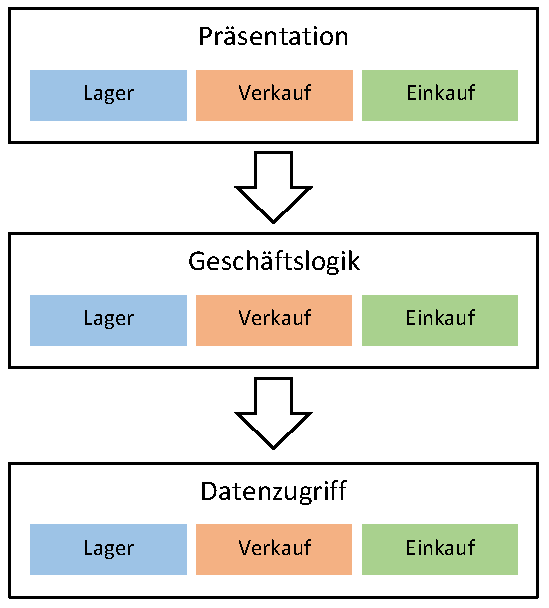
\includegraphics[width=0.8\linewidth]{layered-architecture}
	\caption{Drei-Schicht-Architektur}
	\label{fig:layered-architecture}
\endminipage
\minipage{0.5\textwidth}
  \centering
	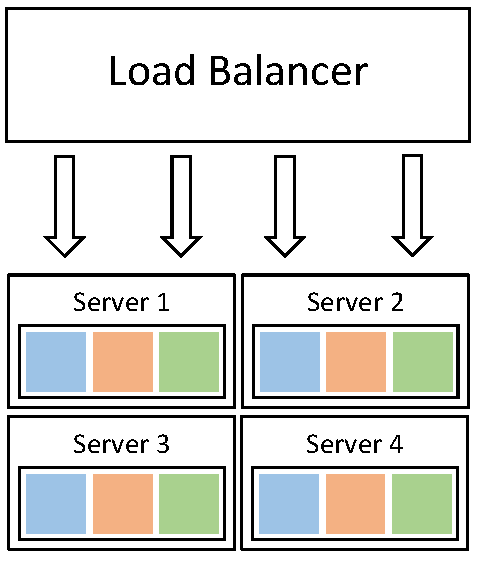
\includegraphics[width=0.76\linewidth]{monolith-scale}
	\caption{Skalieren einer monolithischen Anwendung}
	\label{fig:monolith-scale}
\endminipage
\end{figure}

\subsubsection{Nachteile und Schwierigkeiten}

Mit steigender Komplexität der Software kommen nach und nach Probleme zum Vorschein, die diesen Ansatz aufwändig oder sogar unpraktikabel machen. Eine der größten Herausforderungen bei der Entwicklung von Anwendungen mit globaler Reichweite ist die Skalierbarkeit. Die einzige Möglichkeit eine monolithische Anwendung zu skalieren, ist auf mehreren Servern jeweils eine Instanz der Anwendung zu installieren und über einen Load-Balancer zu verbinden. Abbildung \ref{fig:monolith-scale} zeigt wie ein solcher Aufbau aussehen kann. In vielen Einsatzgebieten ist dieser Ansatz aber nicht feingranular genug. Oft ist es sinnvoller, nur bestimmte Teile des Gesamtsystems zu skalieren.

Ein Monolith stößt aber nicht nur aus technischer Sicht auf Skalierbarkeitsprobleme, sondern auch aus organisatorischer Sicht. Alle Entwickler arbeiten zwangsläufig an der gleichen Codebasis, die dadurch enorme Größe annehmen kann. Kein einzelner Entwickler ist mehr in der Lage, die ganze Codebasis zu überblicken und zu beurteilen, welche Auswirkung eine Änderung haben kann. Das führt über kurz oder lang zur Verlangsamung der Entwicklungsgeschwindigkeit oder sogar zu völligem Stillstand.

Anforderungen an eine Software ändern sich häufig sehr rasch. Agile Softwareprozesse unterstützen dabei, die geänderten Anforderungen zeitnahe in die Software einfließen zu lassen. Für den Kunden \bzw Endbenutzer zählt nur die schnellstmögliche Umsetzung seiner neuen Anforderungen. In einer monolithischen Anwendung sind mehrere Geschäftsbereiche zusammengefasst. Somit muss die Anwendung immer als ganzes getestet und ausgerollt werden. Dadurch verlangsamt sich der gesamte Releasezyklus auf den langsamsten Teilbereich, obwohl vielleicht der geänderte Teilbereich schon längst fertiggestellt ist.

Hinter einer monolithischen Anwendung steht immer eine bestimmte Technologie oder eine Sammlung von mehreren Technologien, wie \zB Java EE oder ASP.NET. Somit müssen alle Teilbereiche der Anwendung auf die selben Technologien zurückgreifen. Für manche Teilbereiche könnte aber möglicherweise die Verwendung von alternativen Technologien und Speichersystemen große Vorteile bringen.

In diesem Abschnitt wurden einige der Hauptkritikpunkte am monolithischen Architekturmuster angeführt. Es mag den Anschein vermittelt haben, dass dieser Ansatz nicht mehr verwendet werden soll oder veraltet ist. Aber das ist so nicht der Fall. Viele Experten sind der Meinung, dass gerade am Anfang eines Projekts der monolithische Ansatz zu bevorzugen ist \cite{FowlerMolithFist}. Erst nachdem das Verständnis für die Domäne vorhanden ist und Anforderungen klarer sind, ist der fließende Übergang zu einer Microservice Architektur einfacher und sinnvoll. 

\section{Charakteristiken von Microservices}

Dieser Abschnitt beschreibt einige charakteristische Merkmale eines Microservices. Wie bereits erwähnt, gibt es keine eindeutige Definition eines Microservices. Daher ist es sinnvoller, allgemeine anerkannte Charakteristiken der Microservice Architektur zu betrachten.
 
\citeauthor{FowlerMS} identifizierte in \cite{FowlerMS} neun Charakteristiken von Microservices. Obwohl diese Liste bereits sehr exhaustiv ist, sind immer wieder sinnvolle Ergänzungen, wie in \cite{HorsdalMS} zu finden. Die nachfolgenden Abschnitte beschreiben eine repräsentative Auswahl dieser Charakteristiken.

\subsection{Organisation um Geschäftskompetenzen}

Normalerweise sind Softwareentwicklungsteams anhand ihrer technologischen Spezialisierung \zB in folgende Teams eingeteilt:

\begin{itemize}
	\item Front-End Entwickler
	\item Backend-End Entwickler
	\item Datenbank-Administratoren
	\item IT-Administratoren
\end{itemize}

Durch die Microservice Kultur hat sich aber eine andere Art der Teamstrukturierung etabliert. Für jede Geschäftskompetenz ist genau ein Team, welches intern aus einer kleinen Anzahl an den eingangs genannten Technologieexperten besteht, verantwortlich. Damit soll die Identifizierung und das Verantwortungsbewusstsein jedes einzelnen Teammitglieds für das von ihm entwickelte und betriebenen Dienstes stärken.

Was aber dennoch eine große Herausforderung bleibt, ist die Definition des Aufgabenbereichs eines einzelnen Teams. Die Identifikation und Abgrenzung der Geschäftskompetenzen eines Unternehmens ist eine sehr komplexe Aufgabe. Als Hilfsmittel lässt sich hier das \begin{english} Single-Responsibility-Principle\end{english} heranziehen \cite{MartinAgile}: 

\begin{english}
\begin{quote}
  \textit{A class should have only one reason to change.}
\end{quote}
\end{english}

Das aus der objektorientierten Programmierung bekannte Entwurfsprinzip kann auch im Kontext von Microservices angewandt werden. Es erweitert diesen Grundsatz von der Klassen-Ebene auf die Dienst-Ebene. Das heißt, jeder Dienst soll genau eine Fähigkeit realisieren. Damit ist sichergestellt, dass geänderte Geschäftsanforderungen so wenig wie möglich andere Microservices beeinflussen.

\subsection{Modularisierung durch Dienste}
\label{subsec:Componentization}

Seit Jahrzehnten strebt die Softwareentwicklungsbranche danach, komplexe Softwaresysteme einfach durch die Integration verschiedener Komponenten realisieren zu können. Durch dieses jahrelange bestreben und unterschiedlichste Ansätze ist leider auch der Begriff Komponente sehr überstrapaziert und hat dementsprechend viele unterschiedliche Bedeutungen. Beispielsweise in der objektorientierten Programmierung, kann eine Klasse als Komponente betrachtet werden. Darüber hinaus gibt es noch viele weitere Bedeutungen.

Auch wenn die konkrete Umsetzung einer Komponente sehr vielfältig sein kann, haben alle Arten die selben Ziele:

\begin{itemize}
	\item \textbf{Austauschbarkeit:} Es soll möglich sein, eine Komponente durch eine andere zu ersetzen. 
	\item \textbf{Wiederverwendbarkeit:} Eine entwickelte Komponente soll auch in anderen Systemen wiederverwendet werden können.
	\item \textbf{Aktualisierbarkeit:} Durch die Austauschbarkeit ist es automatisch möglich, eine Komponente durch eine neuere Version zu ersetzen, ohne den Rest der Anwendung zu beeinflussen.
\end{itemize}

Im Kontext der monolithischen Softwarearchitektur sind am häufigsten die Begriffe Modul oder Software-Bibliothek stellvertretend für den Begriff Komponente. Eine Anwendung besteht somit aus einer Menge von Modulen, die miteinander verbunden sind. Leider erfüllt dieser Ansatz die zuvor beschriebenen gewünschten Eigenschaften der Komponenten-Orientierung nicht ganz zufriedenstellend. Abhängigkeiten zwischen den einzelnen Modulen oder bestimmte Voraussetzungen an das Laufzeitsystem der monolithischen Anwendung können es schnell verhindern, ein Modul zu aktualisieren. Somit sind die verwendeten Komponenten nicht völlig voneinander unabhängig, sondern haben versteckte Abhängigkeiten.

In einer Microservice-Architektur ist mit Komponente ein einzelner Dienst gemeint. Damit ist jede Komponente ein eigener Prozess, der über ein Kommunikationsprotokoll mit anderen Komponenten interagiert. Mit diesem Ansatz lassen sich die gewünschten Eigenschaften viel leichter realisieren.

\subsection{Dezentrale Datenverwaltung}

Eine monolithische Anwendung legt sehr häufig alle persistenten Daten in einer einzigen relationalen Datenbank ab. Jeder Programmteil greift einfach auf die benötigten Daten direkt zu. Dieser Ansatz ist in Abbildung \ref{fig:central-datastore} dargestellt. In einer Microservice Architektur ist dieser Ansatz nicht mehr empfehlenswert. Persistente Daten eines bestimmten Geschäftsbereichs sollen nur von einem einzigen Dienst verwaltet werden. Direkter Zugriff auf diese Daten durch andere Dienste führt zu unerwünschten Abhängigkeiten. Andere Dienste müssen Daten über die öffentliche Schnittstelle des zuständigen Microservices abfragen oder verändern.

\begin{figure}[h]
  \centering
	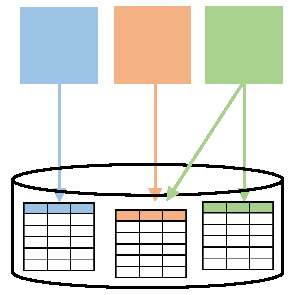
\includegraphics[width=0.3\textwidth]{central-datastore}
	\caption{Zentraler Datenspeicher}
	\label{fig:central-datastore}
\end{figure}

Wenn jeder Dienst wie in Abbildung \ref{fig:polyglot-persistnace} seinen eigenen Datenspeicher besitzt, kann für die Erfüllung seiner Aufgabe der optimale Speichermechanismus ausgewählt werden. Beispielsweise können Daten mit komplexen Beziehungen in einer Graphdatenbank abgelegt werden. Jedoch einfache Daten in einem schnellen Key-Value-Speicher.

\begin{figure}[h]
  \centering
	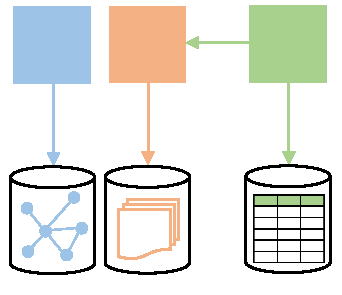
\includegraphics[width=0.3\textwidth]{polyglot-persistance}
	\caption{Polyglot Persistance}
	\label{fig:polyglot-persistnace}
\end{figure}

Auch eine monolithische Anwendung könnte Gebrauch von mehreren Datenbanken machen. Dieser Ansatz ist unter dem Namen Polyglot Persistence bekannt \cite{FowlerPP}. Aus teilweise sehr vielfältigen Gründen ist er aber selten anzutreffen. Nachfolgend nur ein kleiner Auszug:

\begin{itemize}
  \item Die IT-Strategie einiger Unternehmen sehen nur die Verwendung ganz bestimmter Datenbanken vor.
	\item Bereits getätigte Investitionen in bestehende Datenbanken müssen amortisiert werden.
	\item Angst vor dem Betrieb einer Datenbank für die noch nicht die notwendige Erfahrung aufgebaut wurde.
\end{itemize}

Für Systeme mit hohen Anforderungen an die Verfügbarkeit ist die Verwendung einer einzigen Datenbank nicht ausreichend. Denn eine einzige Datenbank stellt einen kritischen \textit{Single Point of Failure} dar.

\subsection{Automatisierung}

Für ein erfolgreiches System das aus Microservices besteht, ist ein hoher Grad an Automatisierung erforderlich. Durch die große Anzahl an Komponenten im System, muss die Anzahl an manuell erforderlichen Schritten sehr gering sein. Ansonsten ist der Aufwand für das Aktualisieren, Ausrollen, Testen und Überwachen viel zu groß.

Um von den Vorteilen der Microservice Architektur gegenüber einer monolithischen profitieren zu können, ist es unabdingbar, dass jeder Dienst einzeln ausgerollt werden kann. Denn nur damit sind die Entwicklungs- und Releasezyklen der einzelnen Dienste im Gesamtsystem voneinander unabhängig.

Wenn jeder Dienst einzeln ausgerollt werden kann, ist es auch möglich, unterschiedliche Versionen gleichzeitig auszurollen. Somit kann eine neue Version getestet werden und erst wenn diese Testphase erfolgreich abgeschlossen ist, der gesamte Datenverkehr auf diesen Dienst umgeleitet werden. Bei Problemen kann schnell der ursprüngliche Zustand wiederhergestellt werden. Insgesamt mindert ein derartiges Vorgehen das Risiko eines großen Big-Bang-Deployments.

Damit dieser Ansatz funktioniert, müssen die Dienste einige Anforderungen erfüllen. Jeder Dienst steht mit einigen anderen in Verbindung. Wenn nun eine neue Version eines Dienstes ausgerollt wird, muss dessen Schnittstelle abwärtskompatibel sein, da seine Konsumenten noch die alte Schnittstelle verwenden. Fehlertoleranz ist eine weitere wichtige Eigenschaft, da während eine neue Version ausgerollt wird, der Dienst kurzzeitig nicht verfügbar sein kann.

\subsection{Größe}

Wie der Name bereits suggeriert, soll ein Microservice klein sein. Das sollte schon durch die Anwendung des \textit{Single-Responsibility} Prinzips aus Abschnitt \ref{subsec:Componentization} gegeben werden. Wie groß ein Dienst genau sein soll, lässt sich aber aus vielen Gründen schwer festlegen. Die Anzahl der Quelltextzeilen ist ein schlechtes Maß für die Größe, da sie je nach Programmiersprache stark variiert. Schon aussagekräftiger ist die benötigte Zeitdauer für die Entwicklung des Dienstes. Aber auch diese Kennzahl kann trügerisch sein. Beispielsweise kann die Verwendung von externen Bibliotheken eine große Zeitersparnis erzielen. Jedoch inkludiert der Service dann auch die Komplexität dieser Bibliothek.

Eine genaue domänen-unabhängige Größenangabe ist praktisch nicht möglich. Es kann lediglich ein grober Rahmen abgesteckt werden. Ein Microservice sollte eine Entwicklungszeit von mehreren Wochen nicht übersteigen.

Neben quantitativen Kennzahlen sind oft subjektive Kriterien erforderlich. Eine davon ist, dass ein einzelner Entwickler die gesamte Funktionalität eines Dienstes noch im Kopf behalten können muss. Sobald es keinen einzelnen Menschen mehr gibt, der alle Aspekte des Dienstes auf einmal überschauen kann, ist er auf jeden Fall zu groß. Meistens aber haben erfahrene Architekten und Entwickler ein sehr gutes Gefühl, ab welcher Größe ein Dienst zu groß ist.

\section{Vorteile}

Ein neuer Softwareentwicklungsansatz setzt sich nur dann durch, wenn er auch einen erkennbaren Mehrwert bietet. Dieser Abschnitt zeigt einige der Vorteile, die durch den intelligenten Einsatz einer Microservice Architektur entstehen können \cite{fowlerMSTradeOffs,newman2015building}.

Es ist wichtig zu verstehen, dass die Vorteile, die durch Microservices entstehen, erst ab einer gewissen Größe \bzw Komplexität des Gesamtsystems zum Tragen kommen. In einfachen Softwaresystemen steht Komplexität der Microservice Architektur in keinem angemessenen Verhältnis zu den Vorteilen \cite{fowlerMSPremium}.

\subsection{Heterogener Technologieeinsatz}

Beim monolithischen Ansatz sind die Technologieentscheidungen äußerst eingeschränkt \cite{fowlerMSTradeOffs}. Nachdem die Haupttechnologie festlegt ist, kann aus diesem Korsett nur noch geringfügig ausgebrochen werden. Aber nicht für alle Aufgaben muss der eingeschlagene Weg auch der optimale sein.

Hier kommt ein wesentlicher Vorteil von Microservices zum Tragen. Da jeder Dienst eine kleine autonome Komponente ist, sind für jeden Dienst unterschiedliche sinnvolle Technologieentscheidungen möglich. Selbst die Wahl des Speichermechanismus kann individuell erfolgen. Die eingesetzte Technologie kann beispielsweise von der Aufgabenstellung oder den Fähigkeiten der Teammitglieder abhängig gemacht werden. Damit werden die Technologieentscheidungen nicht mehr von zentraler Stelle gesteuert, sondern die Kompetenz in die einzelnen Teams verlagert.

Die Macht der freien Technologieauswahl ist aber mit Bedacht einzusetzen. Es kann für ein System auch kontraproduktiv sein, wenn zu viele Technologien eingesetzt werden, die womöglich noch nicht einmal ein stabiles Stadion erreicht haben. Daher macht die Definition von team-übergreifenden Richtlinien zur Technologieauswahl durchaus Sinn. Der entscheidende Vorteil gegenüber dem monolithischen Ansatz ist aber die Wahlfreiheit, auch nach dem Start der Entwicklung.

\subsection{Robustheit}

Durch den hohen Modularisierungsgrad in einer Microservice Architektur herrscht ein ganz anderes Verständnis bezüglich der Verfügbarkeit von einzelnen Komponenten, wie in einer monolithischen Architektur. In einer monolithischen Anwendung befinden sind nämlich alle Komponenten in einem einzelnen Prozess. Daher kann ein Entwickler davon ausgehen, dass alle Komponenten immer verfügbar sind. Nicht so in einer Microservice Architektur. Hier muss jederzeit davon ausgegangen werden, dass Dienste nur eingeschränkt oder gar nicht verfügbar sind.

Wenn eine monolithische Anwendung ausfällt, ist das ganze System nicht mehr verwendbar. Im Gegensatz dazu kann das Gesamtsystem trotz des Ausfalls eines oder mehrere Microservices, zumindest eingeschränkt, weiterlaufen.

\subsection{Einfaches Deployment}

Jedes Release einer großen monolithischen Anwendung stellt ein gewisses Risiko dar. Daher passieren solche Releases in eher großen Abständen. In einem agilen Umfeld sind derartige lange Releasezyklen nicht tragbar. Außerdem kann jede kleine Fehlfunktion das ganze Deployment zum Scheitern bringen.

Mit Microservices ist es möglich jeden Dienst einzeln auszurollen. Damit ist die Auswirkung aus Sicht des Gesamtsystems viel geringer. Wenn der Dienst nach dem Ausrollen einen Fehler aufweist, kann nur dieser eine Dienst auf den Ausgangszustand zurückgesetzt werden.

Auch die Abhängigkeiten zwischen den einzelnen Teams ist durch den Microservice Ansatz reduziert. Ein Team kann ihren Service um Funktionalität erweitern und sofort ausrollen. Andere Teams die diese Funktionalität verwenden wollen, können erst dann neu ausrollen wenn ihr Dienst stabil ist. Dafür ist es aber notwendig, dass alle Dienste ihre Schnittstellen stets Rückwärts-kompatibel halten.

Die in diesem Abschnitt beschriebenen Vorteile einer Microservices Architektur sind keinesfalls allumfassend. Je nach Einsatzgebiet kommen möglicherweise auch andere Vorteile stärker zum tragen als die hier angeführten. Um von den Vorteilen profitieren zu können, ist eine ordentliche Umsetzung dieses Architekturmusters aber unumgänglich. Denn ansonsten hat man zwar die gesamte Komplexität die Microservices mit sich bringen, jedoch nicht die gewünschten Vorteile.

\section{SOA}

Ein kontrovers diskutiertes Thema im Bezug auf Microservices ist die Beziehung zu Service-orientierter Architektur, kurz SOA. Das abstrakte Architekturmuster SOA wurde bereits 1996 in \cite{schulte1996service} beschrieben und hat sich seither ständig weiterentwickelt.

Auch bei SOA ist es schwer, eine genaue Definition zu geben. Grundsätzlich handelt es sich dabei um eine lose gekoppelte Softwarearchitektur, in der die Komponenten der Software in Form von autonomen Diensten, um die Geschäftsprozesse gestaltet werden \cite{soaRW}. Neben dieser einfachen informellen Definition hafteten sich über die Jahre immer neue Konzepte an den Begriff an. Mittlerweile verbinden viele Architekten konkrete Technologien mit dem eigentlich abstrakten Konzept. Sehr häufig zählen dazu Technologien, wie SOAP, WSDL, WS-* Protokolle oder auch Nachrichten-orientierte Middleware Lösungen, wie ESB \cite{fowlerGoTo}. Aus diesem Grund stößt dieses Muster oft auf Ablehnung, da fälschlicherweise viele komplexe Technologien damit in Verbindung gebracht werden.

\citeauthor{newman2015building} beschreibt in \cite{newman2015building} die Beziehung zwischen Microservices und SOA, wie die Beziehung zwischen Scrum und agiler Softwareentwicklung. Wie Scrum eine konkrete Form von agiler Softwareentwicklung ist, können auch Microservices als ein bestimmter Stil zur Implementierung von SOA gesehen werden. Da alle Konzepte einer Microservice Architektur auch in SOA enthalten sind, können Microservices als Teilmenge und Konkretisierung von SOA verstanden werden.

Oft wird SOA dafür kritisiert, viel zu abstrakt und breit gefächert zu sein. Es gibt viel zu wenig konkrete Hilfestellungen, beispielsweise für den Entwurf von Service-Grenzen oder die Bestimmung der Service-Größe. Microservices hingegen wurde für einen bereits existierenden Stil der Anwendungsentwicklung nachträglich geprägt. Bei SOA hingegen wurde zuerst das Konzept definiert.

\section{Zusammenfassung}

In diesem Abschnitt wurden Microservices als um Geschäftskompetenzen entworfene, lose gekoppelte und autonome Dienste in einer service-orientierten Architektur, definiert. Der Begriff Microservices dient als Sammelbegriff für viele Konzepte die sich um dieses Architekturmuster scharen. Im Gegensatz zu SOA, ist die Vorstellung was Microservices sind, viel genauer, obwohl auch Microservices immer noch viel Interpretationsspielraum offen lassen.

Monolithischen Anwendung bündeln sämtliche Funktionalität eines Systems in einem einzigen großen ausführbaren Prozess. Bei der Microservice Architektur stehen wichtige Funktionalitäten als eigenständiger Dienst zur Verfügung. Das ermöglicht großen Teams, die Arbeit an komplexen Aufgaben, ohne sich gegenseitig zu stören. Damit ist es jedem Team selbst überlassen, die optimalen Technologieentscheidungen zu treffen, den Releasezyklus des Dienstes zu bestimmen und den Dienst in robuster Art und Weise zu implementieren.

Den Vorteilen der Microservices Architektur steht aber eine nicht zu unterschätzende Komplexität gegenüber. Beispielsweise die Orchestrierung aller einzelnen Dienste zu einer Einheit stellt eine große Herausforderung dar. Außerdem fließt viel Arbeit in die saubere Definition der Schnittstellen zwischen den Diensten ein. Einfache Anpassungen können schnell ausarten, da sie mehrere Dienste betreffen können. 

Nichts desto trotz hat das Microservice Architekturmuster in vielen Einsatzgebieten seine Vorzüge. Am Beginn einer Microservice Architektur sollte eine ausführliche Aneignung des erforderlichen Domänenwissens stehen. Oft funktioniert das nur durch den Start der Entwicklung mit einer monolithischen Architektur. Das Ziel sollte eine evolutionäre Architektur sein. Eine monolithische Architektur kann mit steigenden Verständnis für die Servicegrenzen leicht in eine Microservice Architektur überführt werden.
\chapter{Serverlose Softwarearchitektur}

Die Bereitstellung und der Betrieb von Software"=Applikationen sind zwei oft unterschätze Kostenfaktoren. Viele technologische Entwicklungen der letzten Jahre, wie etwa Hardware"=Virtualisierung, Automatisierungswerkzeuge für Infrastruktur und Cloud"=Computing haben diese Kosten bereits stark reduziert. Dennoch ist der Einsatz einer selbst verwalteten Infrastruktur aufwändig und erfordert intensive Zusammenarbeit zwischen Entwicklern, IT"=Administratoren und Release"=Managern.

Vor der Bereitstellung einer monolithischen Software steht zuerst die Dimensionierung und Beschaffung der benötigten Hardware"=Infrastruktur durch die IT-Abteilung. Diese muss danach noch an die Bedürfnisse und Voraussetzungen der Software angepasst werden. Die Installation der eigentlichen Software ist oft ein manueller oder halb"=automatisierter Prozess. Das ist langsam und fehleranfällig, aber meistens akzeptabel, denn eine monolithische Software hat lange Release"=Zyklen und besteht aus einem einzigen Artefakt.

Die Verwendung des Microservice"=Architekturmusters verändertet diese Situation völlig. Mit diesem Szenario besteht ein einzelnes Softwaresystem aus einer Vielzahl von kleinen Diensten, die möglichst isoliert voneinander ausgeführt werden. Dazu ist eine sehr flexible und agile Bereitstellung der erforderlichen Ressourcen notwendig.

Mit \textit{Infrastructure-as-a-Service (IaaS)} bieten viele Cloud"=Computing"=Dienstleister die Möglichkeit, Server in wenigen Minuten bereitzustellen. Der Verwaltungsaufwand bleibt trotzdem relativ hoch, weil Betriebssystem"=Updates, IT"=Sicherheit, Netzwerkkonfiguration, \usw in der Verantwortung des Verwenders liegen.

Viele Applikationen benötigen kaum Kontrolle über die Umgebung in der sie ausgeführt werden. Für diesen Fall ist die Verwendung eines \textit{Platform-as-a-Service (PaaS)} Dienstes meistens vorteilhafter. Hier übernimmt der \textit{PaaS}-Betreiber die vollständige Verwaltung auf Hardware- und Betriebssystemebene, sodass der Verwender lediglich seine Anwendung im richtigen Format bereitstellen muss. Als Verwender hat man nur noch die Möglichkeit die Kapazität und Skalierbarkeitseigenschaften seiner Anwendung zu beeinflussen. Die genaue Umsetzung obliegt dem Anbieter dieser Dienstleistung.

Die Grundidee hinter \textit{Serverless Computing} ist dem Softwareentwickler eine Plattform für die Bereitstellung von Diensten zu bieten, ohne dass sich dieser um Server, deren Konfiguration oder Kapazitätsmanagement kümmern muss. Bei \textit{IaaS} und \textit{PaaS} ist das nicht oder nur zum Teil gegeben.

Wie viele Konzepte im Microservice"=Umfeld lässt sich auch serverlose Softwarearchitektur nur schwer abgrenzen. Im nächsten Abschnitt werden die zwei zur Zeit häufigsten Ausprägungsformen näher betrachtet.

\section{Arten serverloser Softwarearchitektur}

Serverlose Softwarearchitektur ist ein sehr junges Konzept, dessen weitere Zukunft noch offen ist. Derzeit haben sich aber schon zwei unterschiedliche Sichtweisen auf dieses Themengebiet herauskristallisiert \cite{ServerlessArchitectures}.

In der älteren Sichtweise beschreibt der Begriff \textit{serverlos} Applikationen die sehr stark auf vollständig verwaltete Dienste von Cloud"=Anbietern zurückgreifen. Darunter fallen beispielsweise verwaltete Datenbanken, Authentifizierungs- oder Benachrichtigungsdienste. Dieser Ansatz ersetzt also einen Großteil der Logik auf der Serverseite durch Dienste von Drittanbietern. Daher hat sich auch die Bezeichnung \textit{Backend-as-a-Service} dafür etabliert. Ein Teil der Applikationslogik muss aber dadurch vom Client übernommen werden. Mit JavaScript und verschiedenen Bibliotheken für die Erstellung von Benutzeroberflächen, lassen sich die dafür benötigten \textit{Rich-Applications} effizient realisieren.

Seit etwa 2014 hat sich die Sichtweise durch die Einführung des Dienstes \textit{AWS Lambda} durch \textit{Amazon} etwas geändert. Dieser Dienst erlaubt es, einfache Ereignis-gesteuerte Funktionen zu schreiben, die in der Cloud in einer zustandslosen Ausführungsumgebung vollständig verwaltet laufen. Die Artefakte die ein Entwickler erstellen muss sind einfache Skript"=Dateien die Funktionen mit der gewünschten Applikationslogik enthalten. Aus diesem Grund ist dieser Ansatz unter dem Namen \textit{Functions-as-a-Service (FaaS)} bekannt. Der folgenden Abschnitt beschäftigt sich intensiv mit dieser neuen Sichtweise auf Serverlose Softwarearchitektur.

\section{Functions-as-a-Service}

Im Grunde erlaubt es \textit{Functions-as-a-Service} kleine Aufgaben in Form von Funktionen zu programmieren und skalierbar, ohne weiteren Aufwand in der Cloud zu betreiben. Der Entwickler kann sich voll auf die Geschäftslogik seiner Applikation konzentrieren und muss sich kaum noch um Infrastrukturaufgaben kümmern.

Wie in den allermeisten Programmiersprachen auch, sind Funktionen in diesem Kontext eine relativ kleine Menge Quelltext die nach einer Aktivierung mit bestimmten Eingaben, Ausgaben produziert. Die Aktivierung erfolgt bei Programmiersprachen durch einen Funktionsaufruf. In \textit{FaaS} hingegen durch das Auftreten bestimmter Ereignisse die der Entwickler festlegen kann. Beispiele für derartige Ereignisse sind folgende:

\begin{itemize}
	\item Dem Hinzufügen eines Eintrags in einer Datenbank oder Warteschlange.
	\item Das Empfangen einer HTTP-Anfrage.
	\item Das Empfangen einer neue Nachricht in einer Nachrichtenorientierten Middleware.
	\item Das auftreten eines Zeitgesteuerten Ereignisses.
\end{itemize}

Eine Funktion ist nur dann sinnvoll, wenn sie auch Ausgaben oder zumindest Seiteneffekte produziert. In \textit{FaaS} können diese wieder sehr vielfältig sein. Meistens ist das Ergebnis die Interaktion mit einem anderen Cloud-Dienst wie \zB:

\begin{itemize}
	\item Dem Hinzufügen oder manipulieren von Daten in einer Datenbank.
	\item Das senden einer HTTP-Antwort.
	\item Das Versenden von Benachrichtigungen oder E-Mails.
\end{itemize}

Die folgenden Abschnitte beschreiben vielversprechende Anwendungsgebiete für \textit{FaaS}. Des weiteren werden die Konzepte \textit{FaaS} und \textit{PaaS} voneinander abgegrenzt.

\subsection{Anwendungsgebiete}

Für \textit{FaaS} gibt es in den verschiedensten Bereichen sinnvoll Anwendungsgebiete. Hauptsächlich werden sie aber für kleine und abgeschlossene Funktionalitäten herangezogen. Beispielsweise eignet es sich sehr gut für die Konvertierung und Validierung von Daten. Eine Funktion kann dabei auf ein bestimmtes Ereignis, \zB dem Hinzufügen eines Elements in einer Warteschlange warten, und danach die gewünschte Funktionalität ausführen. Das Ergebnis der Funktion kann \zB automatisch in eine Datenbank gespeichert oder an ein anderes System gesendet werden.

Microservice- und Cloud-Anwendungen verwenden oft eine große Anzahl von Cloud"=Komponenten wie, verschiedenen Datenspeichern, Warteschlangen und Nachrichtensysteme. Damit alle Einzelkomponenten in Summe ein funktionstüchtiges Gesamtsystem bilden, ist viel Logik für die Verbindung und Administration der Komponenten notwendig. Im Englischen wird diese Art von Logik häufig als \textit{Glue-Clode} bezeichnet, weil er die Einzelteile zum einem Ganzen "`zusammenklebt"'. Die Interaktion mit Cloud"=Komponenten ist also ein essentieller Bestandteil von und ist deswegen ein großer Einflussfaktor auf das Programmiermodell von \textit{FaaS}.

Der Erfolg der Microservice"=Architektur und \textit{FaaS} führte bereits zur Entstehung eines möglicherweise neuen Paradigmas: \textit{Nanoservices} \cite{infoqFaaS}. Bei Microservices stehen einzelne Geschäftsanforderungen im Vordergrund. Mit Nanoservice werden einzelne Geschäftsanforderungen noch weiter auf Funktionsebene heruntergebrochen. Ein Beispiel für einen Microservice könnte ein Dienst für die Abwicklung von Bestellungen sein, mit dem es möglich ist Bestellungen anzulegen, zu ändern oder zu verfolgen. Mit Nanoservices wäre jede einzelne dieser Funktionen ein eigener Dienst.

\textit{Amazon} beschreibt in \cite{AwsMultiTier} wie klassische Drei"=Schicht"=Architektur, \zB Web- oder Mobile"=Anwendungen, mit Serverlosen Technologie umgesetzt werden können . Darüber hinaus eignet sich \textit{FaaS} aber genau so gut für Microservice"=Architekturen. Die Einsatzgebiete sind daher sehr breit, was \textit{FaaS} zu einem mächtigen Werkzeug macht.

Viel Potential besteht in neuen Domänen wie \textit{Internet of Things}, \textit{Chat-Bots} oder \textit{DevOps} \cite{NewStackAzurePreview}. In diesen Bereichen ist die Nachfrage nach kleinen skalierbaren Programmen, die sich einfach entwickeln und betreiben lassen, sehr hoch. Durch die Einfachheit von \textit{FaaS} eignet es sich auch sehr gut für den Prototypenbau.

\subsection{Beziehung zu Platform-as-a-Service}

In vielen Bereichen überschneiden sich die Möglichkeiten von \textit{FaaS} mit denen anderer Technologien wie \zB \textit{PaaS}. Dieser Umstand ist nicht weiter verwunderlich, da \textit{FaaS} auf der Basis von \textit{PaaS} aufbaut. Der signifikanteste Unterschied ist die Ereignis-gesteuerte Funktionsweise von \textit{FaaS}. Funktionen werden nach dem Auftreten eines bestimmten Ereignis nur für die Dauer einer Aktivierung ausgeführt. Daher bezahlt der Verwender auch nur die Anzahl der Aufrufe und die Dauer der Ausführungszeit. Bei \textit{PaaS} ist meistens zumindest eine ständig laufende virtuelle Maschine erforderlich, die auf Ereignisse wart. Das Verursacht Kosten auch wenn die Maschine kaum oder gar nicht genutzt wird.

Skalierbarkeit ist in Cloud"-Computing ein essentieller Faktor. \textit{PaaS} bietet dafür die Möglichkeit, abhängig von Metriken wie Prozessorlast, die Anzahl der Instanzen auf denen die Anwendung ausgeführt wird, dynamisch zu erhöhen oder zu verringern. Dieser Ansatz erfordert bereits sehr wenig manuelles Eingreifen durch einen Entwickler oder Administrator. Aber \textit{FaaS} geht hier noch einen Schritt weiter und erfordert praktisch keine manuellen Handlungen um die Funktion skalierbar zu machen. Es ist die Aufgabe des Cloud"=Anbieters die Funktion automatisch zu skalieren. Weil die Funktionen zustandslos sind, kann man sie einfach beliebig oft parallel ausführen.

Die Verwendung von \textit{PaaS} schränkt Technologieentscheidungen stark ein, weil man sich auf eine konkrete Platform bindet. Bei \textit{FaaS} hingegen ist die Auswahl an möglichen Programmiersprachen sehr breit. Laufend fügen Cloud"=Anbieter neue Sprachen hinzu. Damit ist die Technologieabhängigkeit durch die Verwendung von \textit{FaaS} sehr viel geringer.

\subsection{Markt}

Alle namhaften Cloud"=Anbieter wie Amazon, Microsoft, IBM und Google haben bereits \textit{FaaS}"=Produkte in ihrem Angebot. Die nachfolgenden Abschnitte zeigen die Funktionsweise und Prinzipien anhand von \textit{Microsoft Azure Functions}, da diese Implementierung unter der MIT-Lizenz Open-Source verfügbar ist und somit tiefe Einblicke in die Umsetzung bietet. 

\textit{Amazon AWS Lambda} ist von allen Produkten am längsten am Markt und bietet den größten Funktionsumfang. Jedoch haben auch die anderen Anbieter das Potential und die Nachfrage von \textit{FaaS} erkannt und versuchen seither den Entwicklungsrückstand zu schließen.

Derzeit befindet sich dieses doch recht neue Thema noch stark im Wandel. Es ist sehr wahrscheinlich, dass sich einige Dinge in naher Zukunft verändern werden. Die Grundideen haben aber alle Anbieter ähnlich umgesetzt. Trotzdem unterscheiden sie sich in einzelnen Punkten:

\begin{itemize}
	\item Jeder Anbieter bietet unterschiedliche Programmiersprachen an. Es werden aber laufend neue Sprachen in die Produkte integriert.
	\item Auch wie das konkrete Skalierbarkeitsverhalten aussieht, muss beim jeweiligen Anbieter getestet werden.
	\item Meistens sind nur andere Dienste innerhalb des selben Cloud"=Anbieters mit \textit{FaaS} integriert. Dadurch kann sehr leicht eine starke Abhängigkeit zum gewählten Anbieter entstehen.
	\item Natürlich unterscheiden sich die einzelnen Angebote auch im Preis.
\end{itemize}

Derzeit investieren Cloud"=Anbieter sehr viel in die Entwicklung ihrer \textit{FaaS} Produkte. Das gibt einen Hinweis auf das große Potential dieser Technologie.

\section{Azure Functions}

Im März 2016 veröffentlichte die Firma \textit{Microsoft} eine Vorschauversion ihrer eigenen serverlosen Plattform mit dem Namen \textit{Azure Functions} \cite{AzFunIntro}. Nur ein halbes Jahr später folgte die erste offizielle Version \cite{AzFunGA}. \textit{Azure Functions} ist eine Erweiterung der ohnehin schon sehr umfangreichen \textit{Microsoft} Cloud"=Plattform. Diese Technologie eignet sich vor allem für die ereignisgesteuerte Verarbeitung und Transformation von Daten aus verschiedenen Datenquellen. Das deklarative Programmiermodell von \textit{Azure Functions} ermöglicht eine einfache Interaktion mit Daten- und Ereignisquellen. 

\textit{Microsoft} griff für die Implementierung von \textit{Azure Functions} auf folgende, schon länger in \textit{Microsoft Azure} enthaltene Dienste und Bibliotheken zurück \cite{AzFunJourney}:

\begin{itemize}
	\item \textit{App Service - Web App}
	\item \textit{App Service Plan}
	\item \textit{Site Control Manger (SCM)}
	\item \textit{Web Jobs}
	\item \textit{Web Jobs SDK}
\end{itemize}

Tatsächliche Neuentwicklungen waren folgende notwendig:

\begin{itemize}
	\item \textit{Web Jobs SDK Script}
	\item \textit{App Service - Function App}
	\item \textit{Dynamic Hosting Plan}
\end{itemize}

Die nachfolgenden Abschnitte geben einen Überblick hier aufgelisteten Bestandteile, die Entstehungsgeschichte und Anwendungsmöglichkeiten von \textit{Azure Functions}. Großteils beziehen sich die Grundlagen von \textit{App Services} und \textit{Web Jobs} auf \cite{AzWebEssentials4Devs}.

\subsection{Azure App Service}

\textit{App Service} ist in der \textit{Microsoft Azure} Cloud ein Oberbegriff für Services, die in die Kategorie \textit{Platform-as-a-Service} einzuordnen sind. Diese Services haben eine etwas konsequentere Interpretation von \textit{PaaS} als die älteren \textit{Cloud Services}. Bei einem \textit{App Service} übernimmt \textit{Microsoft} die Verwaltung der Infrastruktur, des Betriebssystems und der Laufzeitumgebungen. 

Ein \textit{App Service} ist einem sogenannten \textit{App Service Plan} zugeordnet. Dieser kann mehrere \textit{App Services} zusammenfassen, die auf einem oder mehreren Servern gemeinsam ausgeführt werden. Der \textit{App Service Plan} ist also eine abstrakte Infrastrukturbeschreibung, welche die Anzahl, Größe und das Skalierungsverhalten der virtuellen Maschinen festlegt. Daher wird er oft als \textit{Server Farm} bezeichnet.

Der nächste Abschnitt beschreibt mit \textit{Azure Web Apps} einen konkreten \textit{App Service}, der ein Grundbaustein hinter \textit{Azure Functions} ist.

\subsubsection{Azure Web App}

Eine \textit{Web App} ist in \textit{Microsoft Azure} der einfachste Weg um eine Web"=Anwendung bereitzustellen. Die virtuellen Maschinen des \textit{App Service Plan} in dem eine \textit{Web App} ausgeführt wird, sind bereits mit den gängigsten Webentwicklungsumgebungen ausgestattet. Damit lassen sich Web"=Anwendungen in unterschiedlichen Technologien gemeinsam betreiben. \textit{Web Apps} sind als eine Abstraktion eines Web"=Servers zu verstehen.

\subsection{Site Control Manager}

Die Funktionalität eines \textit{App Service} und somit auch einer \textit{Web App} ist mit Hilfe sogenannter \textit{Site Extensions} erweiterbar. Diese Erweiterungen werden im selben Kontext wie die eigentliche Web Anwendung ausgeführt. Der \textit{Site Control Manager} -- oft auch \textit{KUDU} genannt -- ist eine Erweiterung die bei jedem \textit{App Service} automatisch vorinstalliert ist. 

Anfänglich war die einzige Aufgabe des \textit{Site Control Manager} die Auslieferung des \textit{App Service} mittels Versionsverwaltungssystemen. Aber im Laufe der Zeit wurden weitere Funktionen ergänzt. Dazu zählt auch die Funktion \textit{Web Jobs}, welche die Abarbeitung von Hintergrundaufgaben ermöglicht. Für kleinere Aufgaben für die eine eigene virtuelle Maschine überdimensioniert wäre, sind \textit{Web Jobs} oft eine wirtschaftlichere Alternative.

\subsubsection{Web Jobs}

Als \textit{Web Job} eignen sich ausführbare Dateien oder unterstützte Skripte. Diese werden als eigener Prozess im Kontext eines \textit{App Service} entweder zeitgesteuert oder kontinuierlich ausgeführt. Damit können Hintergrundaufgaben überschüssige Kapazität ausnützen. Es kann aber auch zu negativen Effekten kommen, denn Hintergrundaufgaben können die Performanz der eigentlichen Web"=Anwendung für den Endbenutzer beeinflussen.

\subsection{Web Jobs SDK}

Die \textit{Web Jobs SDK} ist eine .NET"=Bibliothek für die Implementierung ereignisgesteuerter Hintergrundaufgaben. Das besondere daran ist das deklarative Programmiermodell, dass es erlaubt mit externen Datenquellen zu interagieren, ohne dafür extra Quelltext schreiben zu müssen \cite{WebJobsSdkBindingAttributes}.

Um vorab einen Einblick zu geben, zeigt Programm \ref{prog:webjobssdk} beispielhaft die Verwendung dieser Bibliothek. Der nächste Abschnitt enthält dann eine detailliertere Aufarbeitung der verwendeten Konzepte. Die folgende Aufzählung gibt eine Übersicht wichtiger Aspekte des Einführungsbeispiels:

\begin{itemize}
	\item Die Zeilen \textit{(1-5)} definieren eine Datenstruktur mit drei Attributen.
	\item Zeile \textit{(7)} startet die \textit{Web Jobs SDK} Laufzeitumgebung. Diese sucht per .NET Reflection nach kompatiblen Funktionen.
	\item Zeile \textit{(10)} definiert eine Funktion die ereignisgesteuert aufgerufen wird.
	\item Zeile \textit{(11)} definiert das Ereignis, das einen Funktionsaufruf auslöst. Hier wird die Funktion bei jedem neuen Eintrag in einer Warteschlangen aufgerufen und dessen Inhalt automatisch an den Funktionsparameter übergeben.
	\item Zeile \textit{(12)} definiert einen Ausgangsparameter. Wertzuweisungen an diesen Parameter werden automatisch in dem konfigurierten \textit{Blob Storage} gespeichert. Für den Pfad dieses Eintrags werden die aus dem Parameter in Zeile \textit{(11)} übergebenen Werte extrahiert.
	\item Zeile \textit{(13)} definiert einen weiteren Ausgangsparameter, der an eine andere Warteschlange weitergeleitet wird. Dieses Ereignis könnte wiederum einen anderen Funktionsaufruf auslösen. 
\end{itemize}

\begin{program}[!hbt]
\caption{Web Jobs SDK Beispiel}
\label{prog:webjobssdk}
\begin{CsCode}
  public class SensorData {
    public string SensorId { get; set; }
    public string Timestamp { get; set; }
    public double Value { get; set; }
  }
  class Program {
    static void Main() => new JobHost().RunAndBlock();
  }
  public class Functions {
    public static void ProcessSensorData(
      [QueueTrigger("sensorqueue")] SensorData sensorData,
      [Blob("values/{SensorId}/{Timestamp}")] out string sensorValue,
      [Queue("aggregationqueue")] out SensorData aggregationQueue) {
      sensorValue = sensorData.Value.ToString();
      aggregationQueue = sensorData;
    }
  }
\end{CsCode}
\end{program}

Obwohl die Funktion in Programm \ref{prog:webjobssdk} mit drei verschiedenen externen Datenquellen interagiert, enthält sie dafür fast keinen imperativen Quelltext, sondern lediglich eine deklarative Beschreibung in Form von Attributen. Die eigentliche Interaktion und das Warten auf Ereignisse ist die Aufgabe der \textit{Web Jobs SDK}. 

Eine \textit{Web Job} Anwendungen ist nichts anderes als eine gewöhnliche .NET Applikation mit einer Referenz auf die \textit{Web Jobs SDK}. Der nächste Abschnitt beschreibt wie statische Methoden einer \textit{Web Job} Anwendungen zu einem ereignisgesteuerten \textit{Web Job} werden.

Für viele Einsatzgebiete reicht dieses einfache, deklarative Programmiermodell aus. Es spricht aber nichts dagegen, die Interaktionslogik mit einer Datenquelle selbst im Funktionsrumpf zu implementieren. Das ist oft sogar notwendig, wenn der Funktionsumfang der deklarativen Variante nicht ausreicht. Der Grundgedanke ist jedoch derartigen repetitiven Standardquelltext durch deklarative Programmierung zu vermeiden.

\subsection{Bindungen}

Die zwei wesentlichen \textit{Web Job} Bindungen sind Trigger"=Bindungen und Nicht"=Trigger"=Bindungen. Erstere überwachen eine Ereignisquelle und lösen den Aufruf einer Job Funktion aus, wenn ein Ereignis auftritt. Zweitere binden Parameter einer Job Funktion an eine externe Datenquelle. Das kann sowohl zum Lesen, als auch zum Schreiben von Daten sein. Darum werden Nicht"=Trigger"=Bindungen in Eingangs- und Ausgangsbindungen eingeteilt. Jede Funktion muss genau eine Trigger"=Bindung haben, kann aber beliebig viele Nicht"=Trigger"=Bindungen enthalten.

Es gibt bereits eine Vielzahl vorhandener Bindungen. Entwickler können die Bibliothek aber auch mit selbst oder von Drittanbietern entwickelten Bindungen erweitern. Dazu muss man die wichtigsten dafür notwendigen Klassen kennen. Abbildung \ref{fig:webjobsclassdiag} zeigt den Bindungsmechanismus von Nicht"=Trigger"=Bindungen in einem stark vereinfachten Klassendiagramm.

\begin{figure}[!hbt]%
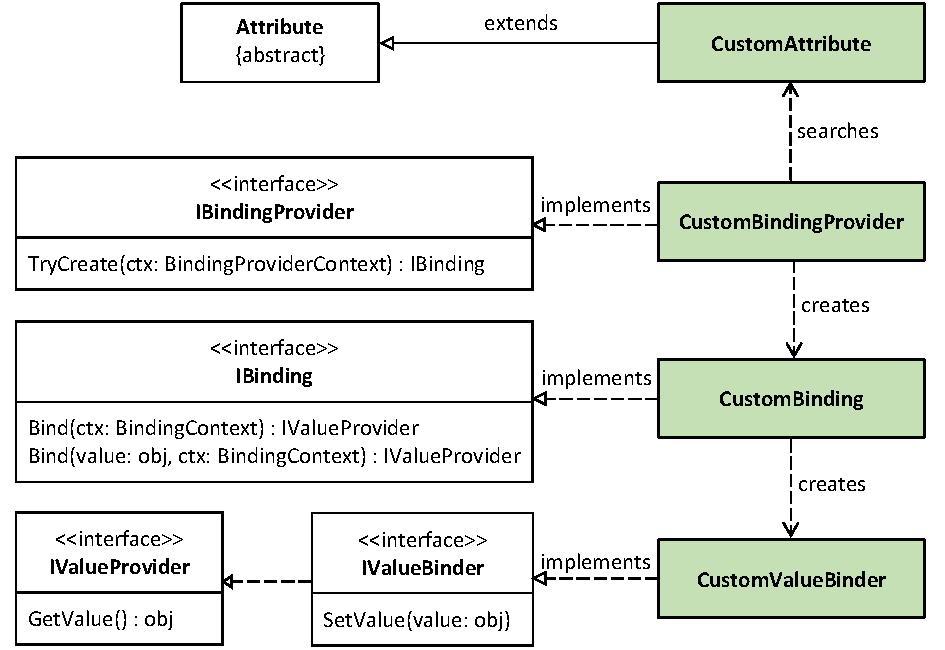
\includegraphics[width=\columnwidth]{webjob-ext-nontrigger-classdiag2}%
\caption{Web Jobs SDK Klassendiagramm (Nicht-Trigger-Bindung)}%
\label{fig:webjobsclassdiag}%
\end{figure}

Wie \cite{WebJobsSdkBindingProcess} beschreibt, ist der Bindungsprozess in zwei Phasen eingeteilt. Die nächsten Abschnitte beschreiben diese Phasen und geben somit auch Aufschluss darüber, wie die in Abbildung \ref{fig:webjobsclassdiag} skizzierten Klassen in Zusammenhang stehen.

\subsubsection{Startphase}

In der erste Phase beim Starten der Anwendung werden alle Funktionen auf ihre Tauglichkeit als \textit{Web Job} untersucht. Dieser Prozess umfasst folgende Schritte:

\begin{enumerate}
	\item Das Assembly der Anwendung wird nach allen Methoden in allen öffentlichen Klassen durchsucht.
	\item Für jeden Parameter einer Methode wird versucht eine Bindung zu erzeugen.
	\item Jeder registrierte \lstinline{I(Trigger)BindingProvider} bekommt die Möglichkeit eine Bindung über die Fabrikmethode \lstinline{TryCreate} zu erstellen. Diese Methode überprüft den Datentyp des Parameters und meistens die Existenz des Bindungs"=Attributs, welchess die Meta-Daten der Bindung beinhaltet. Sind die Voraussetzungen einer konkreten Bindung erfüllt, wird eine Bindung zurückgegeben.
	\item Wenn alle Parameter gebunden werden konnten, wird die Funktion im der \textit{Web Jobs} Laufzeitumgebung registriert.
	\item Für jede Trigger"=Binding wird zusätzlich die Überwachung der jeweiligen Ereignisquelle gestartet.
\end{enumerate}

\subsubsection{Laufzeitphase}

Nachdem alle Funktionen identifiziert wurden, beginnt die Laufzeitphase. In dieser Phase passiert die tatsächliche Bindung der Funktionsparameter. Dieser Ablauf lässt sich wie folgt zusammenfassen:
, wenn ein Funktionsaufruf durch ein Trigger"=Ereignis ausgelöst wurde.

\begin{enumerate}
	\item Ein Ereignis einer Trigger"=Bindung wird beobachtet und führt damit zur Ausführung der assoziierten Job Funktion.
	\item Für jeden gebundenen Parameter wird die \lstinline{BindAsync} Methode der zur Startphase festgelegten Bindung aufgerufen. In dieser passiert der eigentliche Interaktionsschritt mit einer externen Datenquelle, wie \zB dem Lesen von Daten aus einer Datenbank.
	\item Oft unterstützen Bindungen verschiedene Parametertypen, wie \zB \lstinline{String} oder \lstinline{Stream}. Die Bindung muss die tatsächlichen Werte auf den Datentyp der aufzurufenden Funktion konvertieren.
	\item Nachdem alle Parameter gebunden wurden, kann die eigentlich Funktion aufgerufen werden.
\end{enumerate}

\subsection{Web Jobs Script SDK}

Die \textit{Web Jobs Script SDK} ist das Herzstück von \textit{Azure Functions}. Es ist eine .NET Bibliothek, die eine interaktive Verwendung der sonst nur für .NET Applikationen geeigneten \textit{Web Jobs SDK} auch anderen Programmiersprachen zugänglich macht.

Die \textit{Web Jobs SDK} ist eine .NET Bibliothek und daher auch nur für .NET Anwendungen geeignet. Um die schon vorhandene Funktionalität auch für andere Sprachen und Platformen verfügbar zu machen, wurde die Bibliothek \textit{Web Jobs SDK Script} entwickelt.

- No Compilation step needed
- Simply change file - Runtime detects change
- Meta-Data in Attributes -> Meta-Data in Json file
- Folder structure - folder per function -> script files and config file


\subsection{Azure Function App}

Part of app services
Evolution of web jobs
Many languages
Serverless
Groups belonging functions together

- In Azure waren viele Bausteine für eine serverlose Platform bereits vorhanden (Web Jobs, Web Jobs SDK, ...)


\subsection{Verrechnungsmodell}

- GB/s
- Vergleich mit lasttest und dedicated service plan

\subsection{REST-Schnittstellen implementieren}

- Einfach REST implementieren
- Generisch?

\subsection{Kaltstart}

\subsection{Erweiterbarkeit}

\subsection{Zusammenfassung}

Ereignisgesteruert, interation
vieles bereits möglich
erst jetzt wirklich serverless
wann serverless und wann dedicated
kaltstart verbesserungen
lego baukasten

\section{Evolution der Anwendungsentwicklung}

Dieser Abschnitt bezieht sich weitestgehend auf \cite{Cock16EvoFunc} und \cite{Cock17ShrinkingMS} in denen der Autor Adrian \citeauthor{Cock16EvoFunc} die Evolution von monolithischer Software"=Architektur hin zu Microservices und weiter zu ereignisgesteuerten serverlosen Anwendungen beschreibt. Außerdem werden die dafür verantwortlichen technischen und organisatorischen Entwicklungen identifiziert.

Software"=Applikationen haben die Aufgabe Geschäftswerte -- \textit{engl. business value} -- zu generieren. Dazu müssen sie den Benutzern die enthaltene Geschäftslogik zugänglich machen. Eine Funktion kann erst Geschäftswerte erzeugen, wenn sie dem Benutzer tatsächlich zur Verfügung steht. Daher sollte die Minimierung der Zeit zwischen der Erstellung der Geschäftslogik und der tatsächlichen Verfügbarkeit für den Endbenutzer für Unternehmen an oberster Stelle stehen. \citeauthor{Cock16EvoFunc} beschreibt diesen Zusammenhang in folgender Formel:

\begin{center}
\textit{time to value = creation cost + delivery cost}
\end{center}

In der Vergangenheit war die Dauer zwischen der Erstellung und der Auslieferung einer neuen Funktion oft sehr lange. Aufgrund des hohen Aufwands und der zahlreichen Risiken eines neuen Releases, wurden Anwendungen nur in sehr großen Zeitabständen ausgeliefert. Zu dieser Zeit waren monolithischen Anwendung, in Verbindung mit einer oder wenigen zentralen relationalen Datenbanken, der effizienteste Weg Geschäftslogik bereitzustellen. Software"=Design war zu einem großen Teil durch Performanzbedenken dominierten. Die folgenden drei Abschnitte erläutern wie Hardware-Fortschritte, Auslieferungsautomatisierung und organisatorische Veränderungen, diese Probleme verringerten und somit den Weg für Microservices und serverlose Anwendungen ebneten.

\subsection{Automatisierung der Softwareauslieferung}

Vor einigen Jahren war die Bereitstellung von Software noch ein manueller Prozess. Die Beschaffung, Installation, Konfiguration und Aktualisierung von physischen Servern war ein wesentlicher Zeit und Kostenfaktor. Durch diese langsamen Vorgänge wurden nur selten, dafür eine große Menge Geschäftslogik, in einer neuen Softwareversion ausgerollt.

Eine zusätzliche Herausforderung stellte die Kapazitätsplanung dar. Viele Server wurden aufgrund der langsamen Änderungszyklen  vorsichtshalber sehr großzügig dimensioniert. Das führte wiederum zu einer unökonomischen Ressourcenauslastung.

Die Automatisierung von Infrastrukturaufgaben regte ein Überarbeitung festgefahrener Softwareauslieferungsprozesse aus. Werkzeuge wie \textit{Chef} und \textit{Puppet} erlaubten es erstmals, Skripte für die automatische Provisionierung und Konfiguration von Infrastrukturkomponeneten zu erstellen. Zu diesen Komponenten zählen Server, Betriebssystem, Netzwerk, Konfiguration, aber auch die Applikationssoftware selbst. Heute bezeichnet man diese Möglichkeiten als \textit{Infrastructure-as-Code}, weil sich Infrastruktur mittels Quelltext erstellen und manipulieren lässt. \cite[135]{Httermann:2012:DD:2380958}.

Wenn sich Infrasturktur wie Quelltext behandeln lässt, ist es naheliegend, dass auch Softwareentwickler an diesem Prozess teilnehmen. Die Infrastrukturprovisionierung und -verwaltung verlagerte sich allmählich von den IT"= in die Softwareentwicklungsabteilungen. IT"=Abteilungen und Cloud"=Anbieter stellten den Entwicklern nur noch Programmierschnittstellen -- sogenannte APIs -- zur Verfügung, mit denen sie selbst die Infrastruktur nach ihren Bedürfnissen erzeugen und verändern konnten. Diese Zeit- und Kostenreduktion bei der Softwareauslieferung ermöglichten häufigere Releases und viel kleinere Anwendungen. Schlussendlich war das eine der Voraussetzung für die Microservice"=Architektur. Die Auslieferung von Service veränderte sich von einem langsamen und risikoreichen Prozess in einen automatisierten.

Alle Anbieter serverloser Plattformen haben auf die Erfahrungen der Vergangenheit aufgebaut und Automatisierbarkeit von Anfang an berücksichtigt. Softwaresystemen mit einer großen Anzahl von Funktionen wären manuell schwer handhabbar. 

\subsection{Leistungsverbesserung der Hardware}

Erst der technologische Fortschritt der Netzwerkübertragungs- und Festplattengeschwindigkeiten haben den Weg für echte Service"=orientierte Architekturen geebnet. Obwohl die Ideen hinter SOA schon lange existieren, wurden sie aufgrund von Performanzengpässen gar nicht oder nur unzureichend umgesetzt.

Nachrichten-orientierte Systeme bedeuten immer einen gewissen Mehraufwand für die Übertragung und Kodierung der Nachrichten. Die Netzwerkgeschwindigkeit hat sich in den letzten Jahren um das zehn- bis hundertfache gesteigert \cite{IEEEBandwidth}. In der Ethernet Spezifikation \textit{IEEE 802.3-2015} sind Übertragungsraten bis zu 100 Gigabit pro Sekunde spezifiziert.

Eine weitere Erschwernis die für Nachrichtenübertragung waren schwergewichtige, oft XML-basierte, Kodierungsprotokolle wie \zB SOAP. Erst die Entwicklung von leichtgewichtigeren \bzw effizienteren Protokollen, in Kombination mit den um Größenordnungen schnelleren Netzwerkverbindungen, leiteten den Siegeszug von Nachrichten-orientierten Systemen ein.

Auch in der Speichertechnologie passierte durch die Ablösung von magnetischen Festplatten durch \textit{Solid-State} Festplatten ein weiterer essentieller Technologiefortschritt. Magnetische Festplatten sind ihren neuen Konkurrenten vor allem bei zufälligen Lesezugriffen deutlich unterlegen. Diese schlechten Zugriffszeiten waren der Grund für das Design großer monolithischer Datenbanken. Geschäftslogikfunktionen mussten viele Operation in einer Transaktion durchführen, um die langsamen Zugriffszeiten zu kaschieren.

Auf der Basis der sehr schnellen \textit{Solid-State} Festplatten wurden eine Menge neuer \textit{NoSQL} Datenbanken entwickelt. Diese wiederum haben die Dezentralisierung und die in Abschnitt \ref{subsec:polyglot-persistance} beschriebene polyglotte Persistenz der bis dato hauptsächlich monolithischen Applikation vorangetrieben.

Auch Funktionen in \textit{FaaS} machen intensiven Gebrauch von Nachrichtenübertragung und verschiedenen Datenspeichern. Im Grunde transformieren sie Daten, wann immer sie über eine Nachricht oder andere Ereignisse benachrichtigt werden.

\subsection{Organisatorische Veränderungen}

Abschnitt \ref{sec:business-capabilities} hat bereits beschrieben, dass Microservices eine Umstrukturierung der Entwicklungsteams zur folge hatte. Projekt- oder Technologie"=bezogene Strukturen wurde in Produkt-bezogene transformiert. Sehr große Teams wurden in viele kleine Teams zerlegt, um den hohen Koordinationsaufwand zu reduzieren. Jedes der Teams ist für den gesamten Lebenszyklus eines oder mehrerer Dienste verantwortlich. Diese Struktur erlaubte eine viel agileren Entwicklung und erfordert weniger definierte Prozesse.

\subsection{Von Microservices zu serverlosen Anwendungen}

Wenn man Microservices auf die Spitze treibt, erfüllt jeder Service nur noch eine einzige Aufgabe. Aufgrund der großen Anzahl von Services in einer Microservice"=Architektur, erfordert dieser Ansatz eine extrem effiziente Bereitstellung von Services. Selbst automatisch erstellte virtuelle Server und Container sind dafür ungeeignet. Für diese Anforderung ist \textit{Function-as-a-Service} eine gute Wahl, denn Funktionen lassen sich in Bruchteilen einer Sekunde ausrollen.

Viele Services werden nur selten oder sehr unregelmäßig genutzt. In diesen Szenarien ist es schwierig mit Containern oder virtuellen Maschinen die Kapazität zum richtigen Zeitpunkt bereitzustellen. Die Auslastung der Ressourcen ist in solchen Fällen meistens nicht optimal. \textit{Function-as-a-Service} ist sehr gut für volatile Lastaufkommen geeignet. Anstatt Rechenkapazität dezidiert zu reservieren, werden Funktionen erst bei Bedarf ausgerollt.

Funktionen enthalten beinahe ausschließlich Geschäftslogik. Es ist kaum Standard- oder Plattform"=Quelltext notwendig. Damit gelingt es Entwicklern oft binnen weniger Tage Funktionen zu entwickeln. Dabei verbinden sie einfach eine Funktion mit anderen Funktionen oder anderen Drittanbieter"=Diensten. Ein großer Vorteil von \textit{Function-as-a-Service} ist, dass die entwickelten Funktionen automatisch hoch skalierbar und hoch verfügbar sind.

Alle zuvor beschriebenen Eigenschaften machen \textit{FaaS} zu einer wertvollen Ergänzung der Microservice"=Architektur. Es gibt aber durchaus Szenarien in denen es nicht gut geeignet ist, beispielsweise wenn die Last sehr groß und vorhersehbar ist.

% INDEX

\iffalse
Serverless
- Intro
  - What
	- Why
	- Amazn
	- OSS
	- Competitors
- App Service Plan
- Kudu (Jobs, Deploy, Kinds, Scripts)
- Web Jobs SDK
  - Glue code
	- Locally / Dashboard
	- Core Arch
- Functions
  - Script Host Architecture
	- Dynamic Plan
	- Scaling
	- Threading
- Perf Benchmarks
- Pricing Comparison
\fi

%%% REMOVE TODO
%\iffalse

TODO:

- Remove todo from _MaSE_PHaider.tex
- Gute MS Def: http://martinfowler.com/microservices/

Weitere Vorteile von Microservices
- Scaling indipendently
- Strong module boundaries
- Organizational structure

- Kapitel mit Voraussetzungen über Microservices
  - ... GOTO Talk von Fowler (Ganz am Ende)

- Kapitel über CAP-Theorem (Consistency, Availability und Partitiontoleranz)

\fi

%%%----------------------------------------------------------
\appendix                                            % Anhang 
%%%----------------------------------------------------------

% Empty

%%%----------------------------------------------------------
\MakeBibliography                        % Quellenverzeichnis
%%%----------------------------------------------------------

%%% Messbox zur Druckkontrolle ------------------------------
%\chapter*{Messbox zur Druckkontrolle}



\begin{center}
{\Large --- Druckgröße kontrollieren! ---}

\bigskip

\Messbox{100}{50} % Angabe der Breite/Hoehe in mm

\bigskip

{\Large --- Diese Seite nach dem Druck entfernen! ---}

\end{center}



%%%----------------------------------------------------------
\end{document}
%%%----------------------------------------------------------